\part{Analyse acoustique du théâtre d'Orange}
\label{part3}

\chapter*{Introduction}
	\addcontentsline{toc}{chapter}{Introduction}
	
%\section{Interface utilisateur} \label{sect_add-on}
 Il est d'usage de prétendre que l'acoustique des théâtres antiques est excellente et que le son, par de simples astuces géométriques, est bien perçu à toutes les places. Il est bon de constater que les romains adaptaient leurs architectures aux usages des bâtiments. Ainsi on pourra distinguer les théâtres antiques des \glspl{odeon} qui, plus petit et complètement fermés avaient un usage exclusivement musical. Les romains ainsi que les Grecs ont choisi de bâtir un type de bâtiment adapté aux représentations théâtrales et ont reproduit de manière assez similaire cette architecture globale en différents lieux. Quelles étaient donc les astuces architecturales permettant d'optimiser la propagation du son sachant que "les architectes [de l'antiquité] n'ont jamais disposé que de deux moyens : la géométrie et l'oreille" \cite[p.15]{canac} ? On sait par ailleurs que l'acoustique faisait parti des préoccupations des architectes puisque Vitruve, contenporain de l'époque Augustéenne en fait réguliérement dasn son livre V. \cite[Livre V]{vitruve}. François Canac, a mené durant de nombreuses années une large étude théorique et expérimentale sur l'acoustique des théâtres antiques \cite{canac}. Il explique que la l'excellente acoustique des théâtres antiques tel que celui d'Orange est dû à plusieurs facteurs géométriques :
\begin{itemize}
\item L'orchestre qui fonctionne comme un miroir et réfléchi le son provenant de la scène vers les gradins.
\item Le mur de scène qui réfléchi également le son vers les gradins. Pour que ce son réfléchi ne soit pas présent sous forme d'écho (ce qui nuirai grandement à la compréhensibilité) il est nécessaire que la scène soit peu profonde. Effectivement, un écho apparait op. 
\item Par ailleurs des murs de scène s'élevaient presque toujours là où le terrain arrière était horizontal avec donc la possibilité de présenter des bruits parasites. Le mur semble donc avoir un rôle de "parason" \cite[p.38]{canac}.
\item L'angle des gradins qui augmente en générale lorsqu'on s'éloigne de la scène et qui permet à tous les spectateurs de bénéficier des réflexions sur l'orchestre \cite[p.103-109]{canac}.
\item Le caractère simple de la géométrie : des murs très réfléchissants des gradins à ciel ouvert permettant la presence de premières réflexions et peu de réverbération \cite[p.33]{canac}.
\item Le \gls{pulpitum} qui présente des niches alternativement rectangulaires et semi-circulaire (mais qui est plat dans les \glspl{odeon}) pourrait servir soit à disperser les échos nuisibles soit à faire résonner la musique \cite[p.38]{canac}.
\item Les gradins doivent permettre à l'acteur de s'entendre en retour afin d'avoir la sensation que sa voix porte \cite[p.42 - tab.II-4]{canac}
\end{itemize}
L'un des caractère essentiel de l'étude acoustique dans un théâtre est la compréhensibilité. Cependant, ne disposant que de peu de données dans ce domaine, nous ne n'étudierons pas ce paramètre. Effectivement, l'usage de la parole dans les représentations théâtrales est difficile à comprendre. Outre le fait que l'élocution était probablement très différente de celle qu'on connait aujourd'hui (Aristote \cite[Chap IV - XIV]{aristote} et Plutarque ont insisté sur l'entrainement rigoureux des acteurs pour développer leur voix et leur aisance sur scène \cite[p.39]{canac}) les acteurs portait probablement des masques amplificateurs pour amplifier leur voix \cite[p.362]{arnaud}. Il est rapporté par Philostrate dans \textit{La vie d'Apollonios de Tyane}, V, 9 "qu'un acteur tragique se rendit en occident et y fit une tournée ... Arrivé à Hyspalis (Seville) il sembla aux indigènes déjà effrayant par son aspect,cbien qu'il n'eût pas encore prononcé une parole sur la scène. En le voyant marcher à grand pas, la bouche démeusurement ouverte, monté sur des chaussures d'une hauteur extraordinaire , le corps dissimulé sous un étrange accoutrement, ces gens, n'étaient pas rassurés; mais quand il se mit à élever la voix et à déclamer sur un ton éclatant, la plupart prirent la fuite, comme poursuivis par les cris d'un démon. Il résulte donc de ce passage que la voix atteignait une sonorité considérable" \cite[p.43]{formige}. Il n'est pas impossible que certains spectacles de théâtre aient été non verbaux et plutôt de type pantomime.
	

Dans ce chapitre nous allons tenter d'aller plus loin dans l'analyse acoustique des théâtre antique en utilisant des outils numériques. Effectivement, nous disposons désormais d'une maquette virtuelle du théâtre d'Orange ainsi que d'un outil de simulation acoustique, nous allons donc pouvoir combiner les deux pour tester différentes hypothèses archéologiques. Quelle était l'impact de la position des spectateurs dans les gradins ? Le toit ou le \gls{velum} avaient-ils une incidence sur le son perçu ? Quels rôles jouent et jouaient les différents matériaux ? Voici quelques exemples auxquels nous tenterons d'apporter des réponses. Le premier chapitre présente comment utiliser le logiciel de calcul acoustique et comment le paramètrer pour la maquette virtuelle du théâtre d'Orange. Des calcul seront ensuite effectuer pour différentes configuration du théâtre afin de tenter d'éclairer certaines hypothèses de reconstitution. Nous verrons dans un contexte plus général comment se situe le théâtre d'Orange par rapport à d'autres théâtres en terme d'acoustique.	
	
\chapter{Configuration initiale}
	\citationChap{
	Les idées sont comme des êtres vivants. Elles naissent, elles croissent, elles prolifèrent, elles sont confrontées à d'autres idées et elles finissent par mourir.
	}{Bernard Werber}
	\minitoc
	\newpage
	
	\section{Utilisation générique du logiciel}
	
La force de ce développement logiciel est que l'utilisateur n'a pas besoin d'effectuer de manipulations complexes pour obtenir les résultats de calcul d'acoustique de salle. Il pourra travailler directement sur son maillage dans le logiciel \gls{cao} et lancer le calcul. Blender permet de développer des scripts en Python qui peuvent par la suite être installés sous forme de \textit{add-on}. L'interface homme-machine de Blender est donc complètement modulable et personnalisable. Un \textit{add-on} a donc été développé dans le cadre de ce projet et son rôle est de fournir un maillage adapté à un outil de calcul externe puis de réimporter les résultats dans Blender pour pouvoir les visualiser (voir fig. \ref{logiciel}). Le coeur du calcul s'effectue sur un programme séparé développé en C++ (via Qt creator). L'utilisation d'un langage compilé permet d'optimiser le temps de calcul et le fait d'être un programme séparé permet aux utilisateurs réticent à utiliser Blender pour pouvoir tout de même s'en servir. Il suffit de placer un fichier de maillage au format \gls{obj} dans le répertoire adéquate pour pouvoir lancer le calcul. A noter que le format \gls{obj} permet d'obtenir les informations sur les vertices, les normales et les faces ainsi que les matériaux. D'autres formats de maillages pourront être implémentés dans un développement futur.

\begin{figureth}
	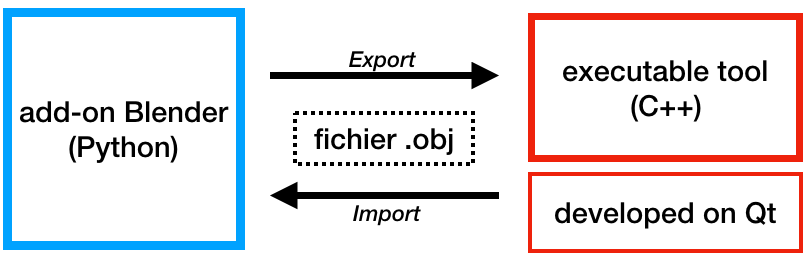
\includegraphics[width=0.7\linewidth]{images/logiciel}
	\caption{Communication entre l'add-on Blender et l'outil de calcul}
	\label{logiciel}
\end{figureth}


Le add-on développé dans la cadre de ce projet possède quelques boutons (voir fig \ref{add-on}). La première étape consiste à notifier le répertoire de donnée de l'outil de calcul afin de pouvoir exporter le fichier de maillage. En utilisant le bouton "Run", Blender transforme les faces des objets sélectionnés en triangles et les exporte au format \gls{obj}. Dans le fichier de maillage, chaque objet est différencié par un en-tête comprenant son nom. S'en suit les coordonnées de l'ensemble de ses sommets (ou vertices), de ses textures et de ses normales. Ensuite sont regroupées par matériaux, les faces par combinaison de trois vertices, d'une texture et d'une normale. Un vecteur de sommets et un vecteur de normales sont remplis face par face en conservant le même ordre. Ces deux vecteurs stockent ainsi la totalité du maillage. Les textures quant à elles ne nous sont pas utiles. Les coefficients d'absorption des matériaux sont aussi assemblés dans un vecteur en les classant face par face en respectant l'ordre établi précédemment. Par défaut, une source et un récepteur sont positionnés au point [0, 0, 0]. Le rayon de mesure du récepteur est de 1m. Cependant, l'utilisateur pourra changer ces paramètres en créant des objets source et récepteur dans Blender. Pour être reconnus et discriminés du maillage, ces objets doivent respectivement comporter les mots "\textit{source}" et "\textit{listener}" dans leur nom. L'algorithme déterminera alors le centre des objets sources et des récepteurs en calculant la moyenne des coordonnées des sommets. Le rayon de mesure du récepteur correspond au rayon de la sphère circonscrite à l'objet "\textit{listener}". Notons qu'il est possible de placer plusieurs sources. L'ensemble des calculs se réaliseront séquentiellement pour une source après l'autre. Un seul récepteur est pris en compte. L'add-on Blender permet de mettre à jour uniquement les informations sur les sources et récepteurs sans avoir besoin de recharger tout le maillage. 
\begin{figureth}
	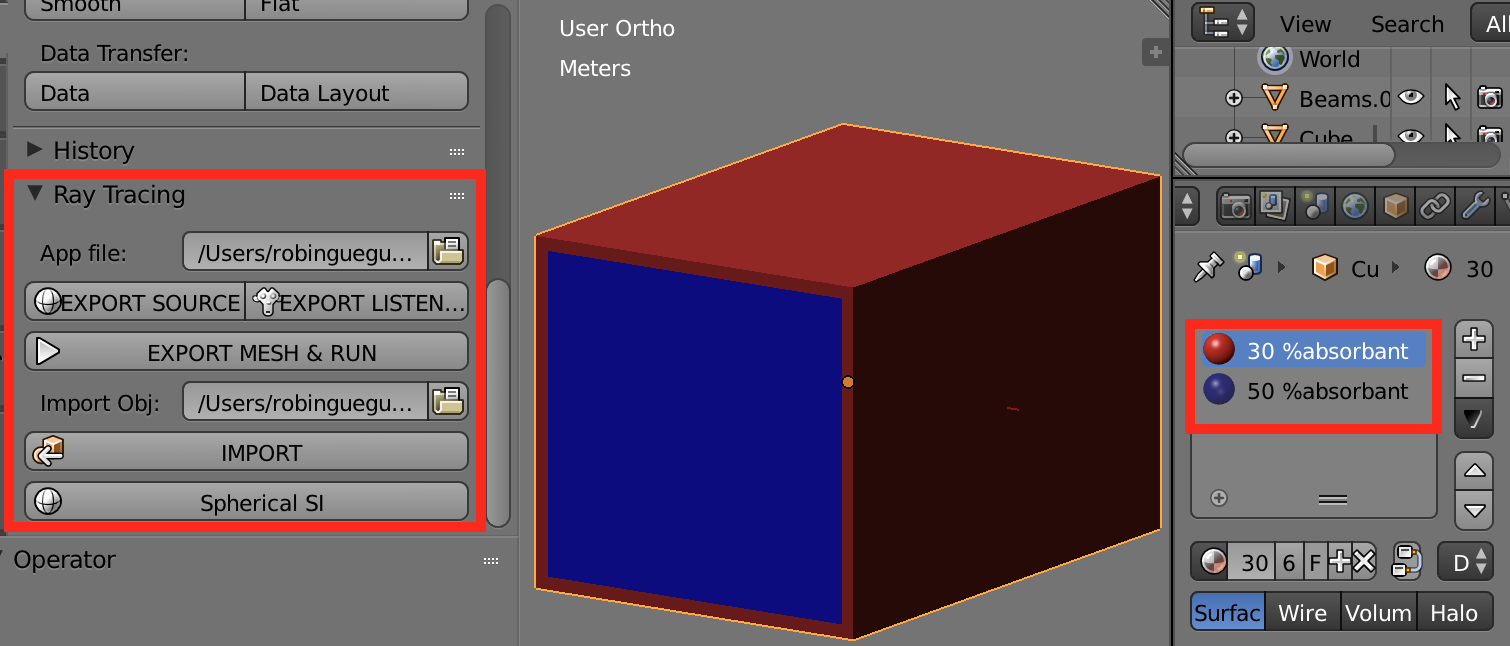
\includegraphics[width=\linewidth]{images/add-on}
	\caption{Add-on Blender et assignation des matériaux}
	\label{add-on}
\end{figureth}
Par ailleurs l'utilisateur assignera aux différentes parois un type de matériau en faisant apparaitre dans son nom la référence du matériau issue de la base de donnée Odéon (voir section \ref{sect_lectMat}). De nombreux autres paramètres sont configurables grâce à une \gls{ihm} générée par Qt (voir fig. \ref{ihm}). On peut alors paramètrer la température, la pression relative, le nombre de rayons, etc. L'outil permet donc d'afficher la \gls{rir} et d'écouter un fichier audio révérberé grace au calcul effectué. Il est ensuite possible de visualiser certains résultats directement sur Blender comme les rayons ou les sources-images par exemple (voir fig \ref{import}). Un option permet aussi de projeter les sources-images sur les parois de la salle afin de visualiser de manière plus intuitive d'où proviennent les reflexions (voir fig \ref{projete}).
\begin{figureth}
	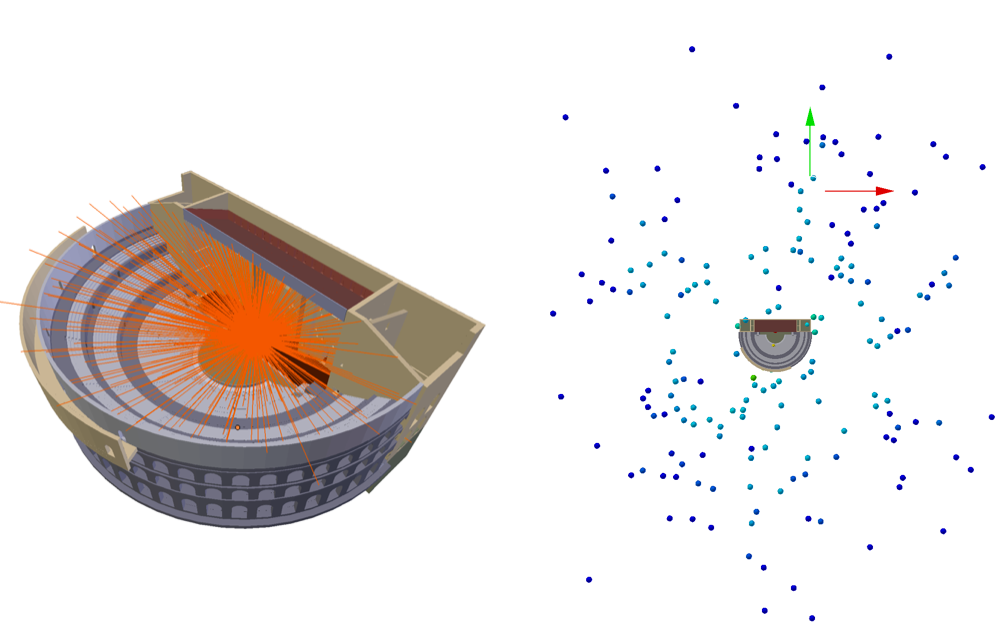
\includegraphics[width=\linewidth]{images/import}
	\caption{Affichage des rayons (une itération) et des sources-images (-60dB) dans le théâtre d'Orange}
	\label{import}
\end{figureth}


\begin{figureth}
	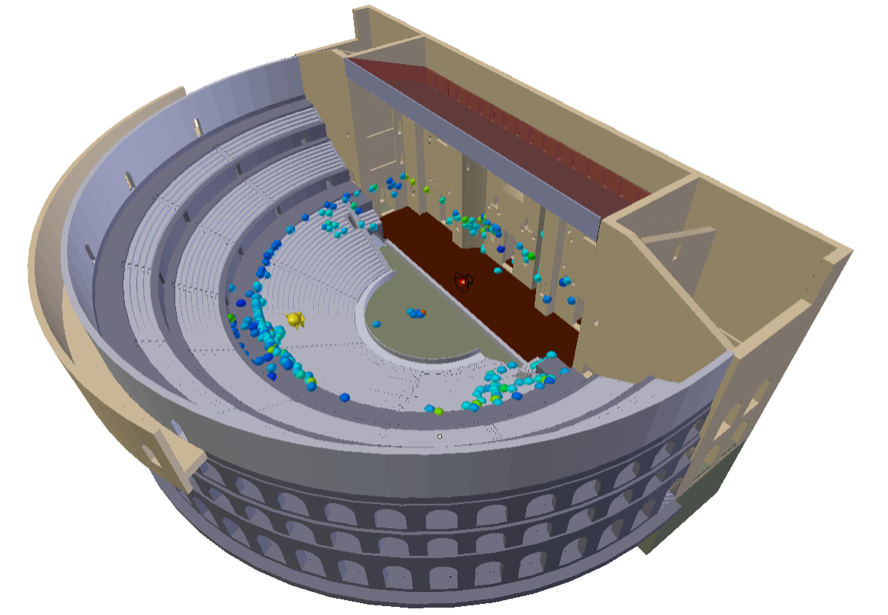
\includegraphics[width=0.8\linewidth]{images/projete}
	\caption{Projeté des sources-images sur les parois du théâtre d'Orange}
	\label{projete}
\end{figureth}


	\section{Configuration du maillage}
Pour effectuer les tests nous mettons en place une configuration de référence.	Ainsi, nous ne conservons que les surfaces à géométrie simple, c'est à dire le mur de scène sans sa décoration, l'\gls{orchestra}, la scène, les basilliques, les \glspl{aditus} et la \gls{cavea} sans la \gls{porticus isc}. On conserve néanmoins les portes et encastrement du mur de scèneEn ce qui concerne les matériaux, nous avons tenter de se rapprocher de la réalité d'après les éléments disponibles aujourd'hui. Tout ce qui est construction en grand appareil est en calcaire de Courthezon \cite[p.43]{orangeTxt}. L'orchestre était à priori dallé avec un matériau de type marbre \cite[p.337]{orangeTxt}. Il en est de même pour le front du \gls{pulpitum} tandis que le plancher était à priori en bois (probablement du chêne pour ses propriétés mécaniques et sa présence régionale). Le front de scène, derrière sa décoration était orné de panneaux mêlant probablement du marbre varié et polychrome ainsi que des mosaïques. Nous assignerons donc dans un premier un matériau de type marbre à l'ensemble du front de scène. Enfin, la configuration initiale se fait avec le public puisque c'est le cas d'utilisation le plus courant, on assigne donc aux gradins un matériau de type audience tout comme aux trois gradins de bois situés sur l'orchestre et réservés au Sénateurs. Ceux-ci ne font pas partie de la modélisation décrite en partie \ref{part_1} car il s'agit de siège mobiles pour lesquels nous ne disposons que de peu d'information. "Dans les théâtres de Rome les sénateurs étaient placés immédiatement avant les chevaliers. Or, à Orange, la place des chevaliers est déterminée par une inscription deux fois répétée sur le premier gradin inférieur du premier \gls{maenianum} : EQjG-III. Il fallait donc que les décurions fussent avant eux, c'est-à-dire sur les gradins de l'orchestre" \cite[p.46]{formige}. Dans la base de donnée Odéon \cite[materials]{odeon} on trouve les matériaux qui se rapprochent le plus de ceux évoqué précédemment et on obtient les coefficients d'absorption correspondant (voir tab. \ref{matOdeon}). Ce qui saute aux yeux dans ce tableau c'est que le calcaire et le marbre sont extrêmement réfléchissant et semble tenir une fonction de miroir acoustique. A contrario le public est plutôt absorbant et on imagine que sont rôle sera de limiter les échos. Quant au bois, il absorbe moyennement les basses fréquences et peu les hautes fréquences.
%
\begin{tableth} 
\footnotesize
	\begin{tabular}{| c | c | m{2cm} | *{8}{c|}}
		\hline
		Matériau &Référence & Equivalent Odéon & 62,5Hz & 125Hz & 250Hz & 500Hz & 1kHz & 2kHz & 4kHz & 8kHz \\
		  \hline
		  \hline
		   Calcaire & 1001 & Smooth brickwork with flush pointing\footnotemark & 0.02&	0.02&	0.03&	0.03&	0.04&	0.05&	0.07&	0.07 \\
		   \hline
		Marbre &2001 & Marble or glazed tile\footnotemark & 0.1 & 0.1 & 0.1 & 0.1 & 0.1 & 0.2 & 0.2 & 0.2 \\
		   \hline
		Bois & 3000 & Hollow wooden podium\footnotemark & 0.4&0.4&0.3&	0.2&	0.17& 0.15& 0.1&	0.1 \\
		   \hline
		Public & 11009 & Audience, lightly upholstered seats\footnotemark & 0.51&	0.51&	0.64&	0.75&	0.8&0	0.82&	0.83&	0.83 \\
	     \hline
	     		Sénateurs & 11003 & Audience on wooden chairs, 1 per sq. m\footnotemark & 0.16 & 0.16 & 0.24 & 0.56 & 0.69 & 0.81 & 0.78 & 0.78 \\
	     \hline

	 \end{tabular}
	\caption{Matériaux et les coefficients d'absorption correspondant du théâtre d'Orange}
	\label{matOdeon}
\end{tableth}
\addtocounter{footnote}{-1}
\footnotetext{Bobran, 1973}
\addtocounter{footnote}{-1}
\footnotetext{Harris, 1991}
\addtocounter{footnote}{-1}
\footnotetext{Dalenbäck, CATT}
\addtocounter{footnote}{1}
\footnotetext{Beranek, Hidaka, 1998}
\addtocounter{footnote}{1}
\footnotetext{Meyer, Kunstmann, Kuttruff, 1964}

\begin{figureth}
	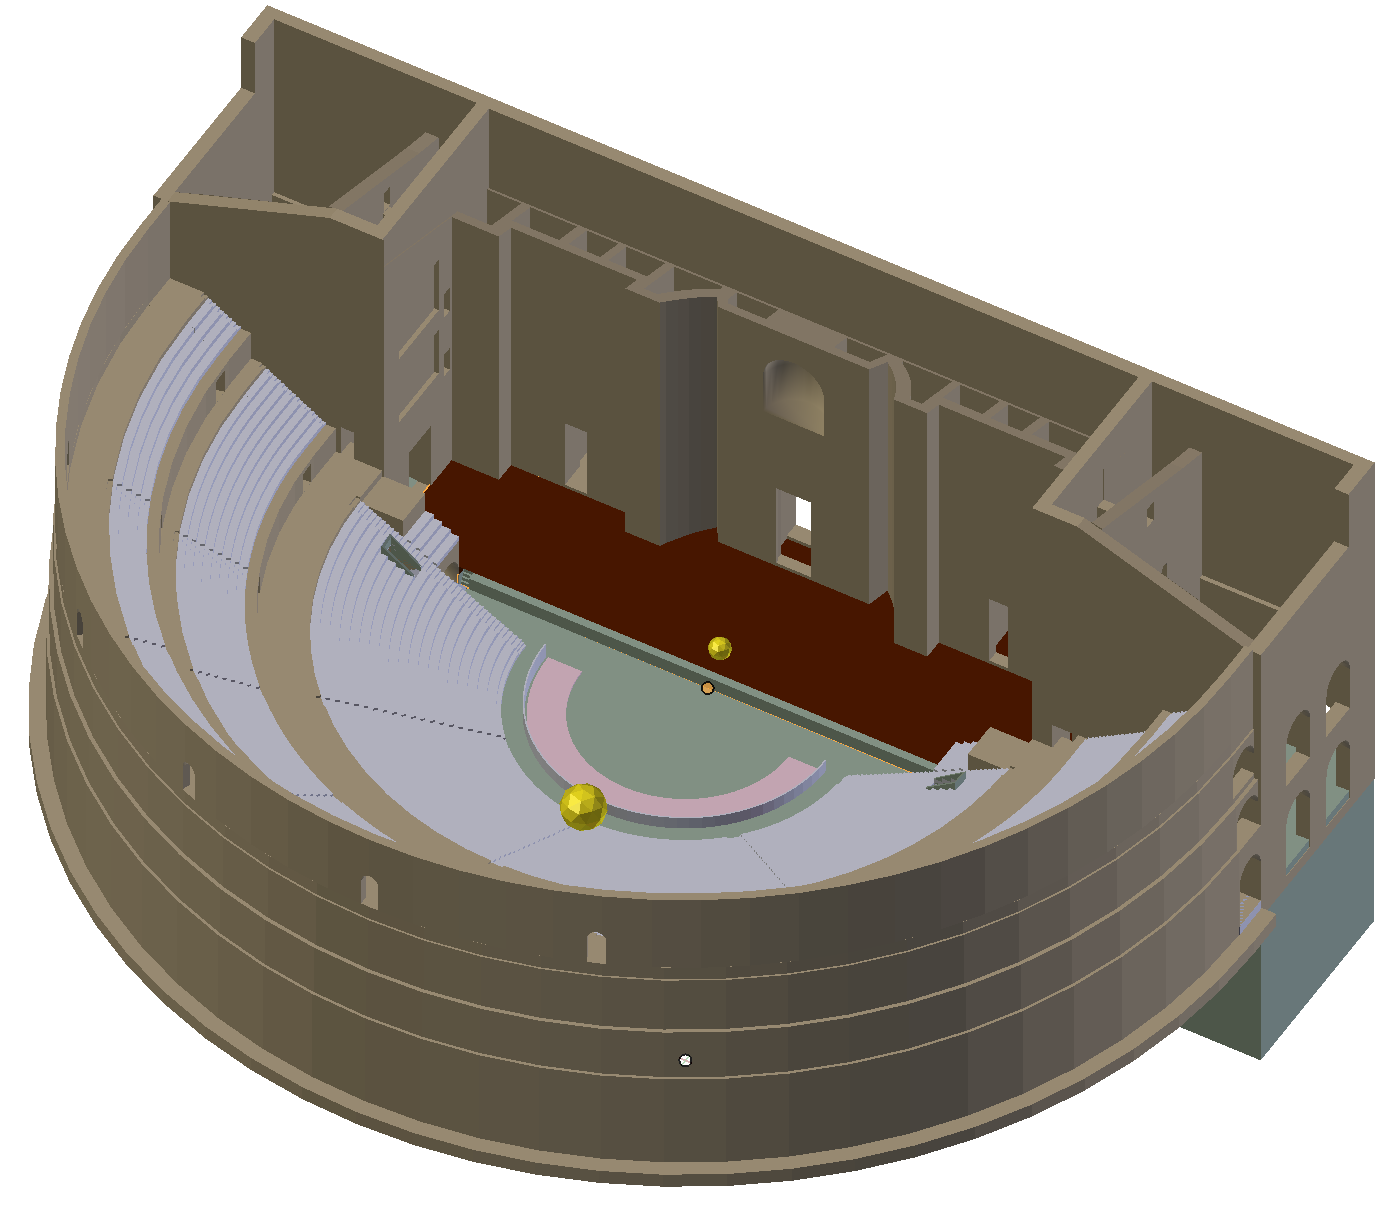
\includegraphics[width=0.7\linewidth]{images/theatreMat}
	\caption{Représentation des matériaux sur le théâtre d'Orange : Calcaire (beige), Marbre (vert), Bois (marron), Audience (gris), Sénateurs (rose) ainsi que la source et le récepteur de la configuration initiale.}
	\label{theatreMat}
\end{figureth}

On peut voir sur la figure \ref{theatreMat} la répartition des différents matériaux sur sur le bâtiment. Nous plaçons une source sonore centrée sur la largeur de la scène à 160cm au dessus de celle-ci (environ la hauteur d'une bouche humaine) soit à une altitude de 42,8m et à 2m du bord. Nous choisissons cette position comme position de source initiale. Le récepteur initial est situé dans le même axe, c'est à dire au centre des gradins et à la même altitude. Sa distance par rapport au centre de l'orchestre est de 16,5m, ce qui correspond aux gradins 3 à 8 environ. Son rayon de mesure sera de 2m. La \gls{rir} de cette configuration pour un \gls{RT60} est présentée figure \ref{rirTheatre}.

\begin{figureth}
	\begin{subfigureth}{\linewidth}
		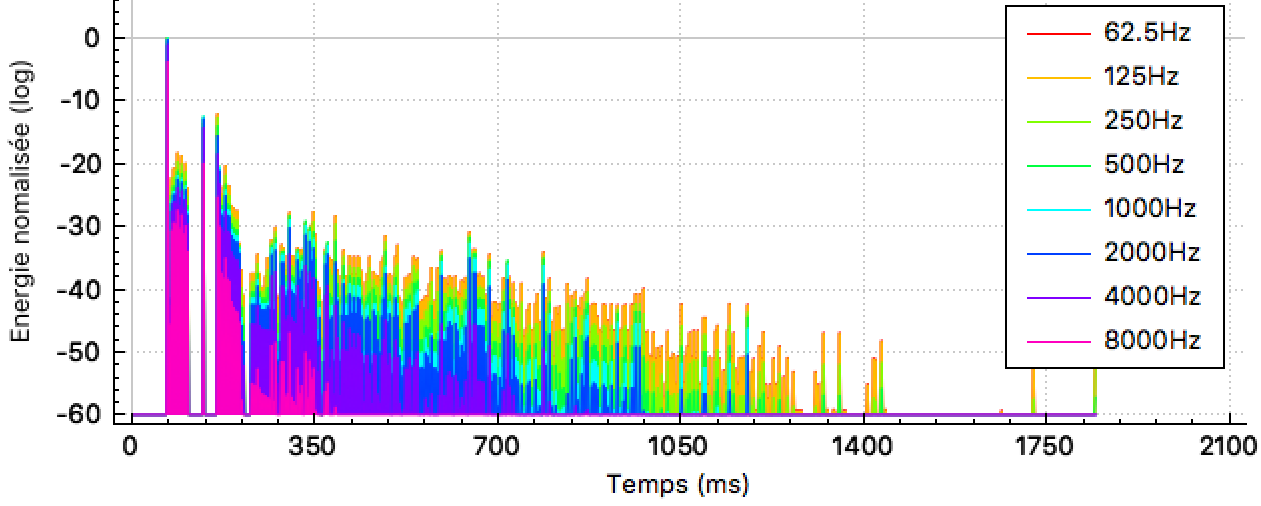
\includegraphics[width=\linewidth]{images/rirTheatre}
			\caption{Figure jusqu'à -60dB}
		\label{rirTheatre60}
	\end{subfigureth}
	\begin{subfigureth}{\linewidth}
		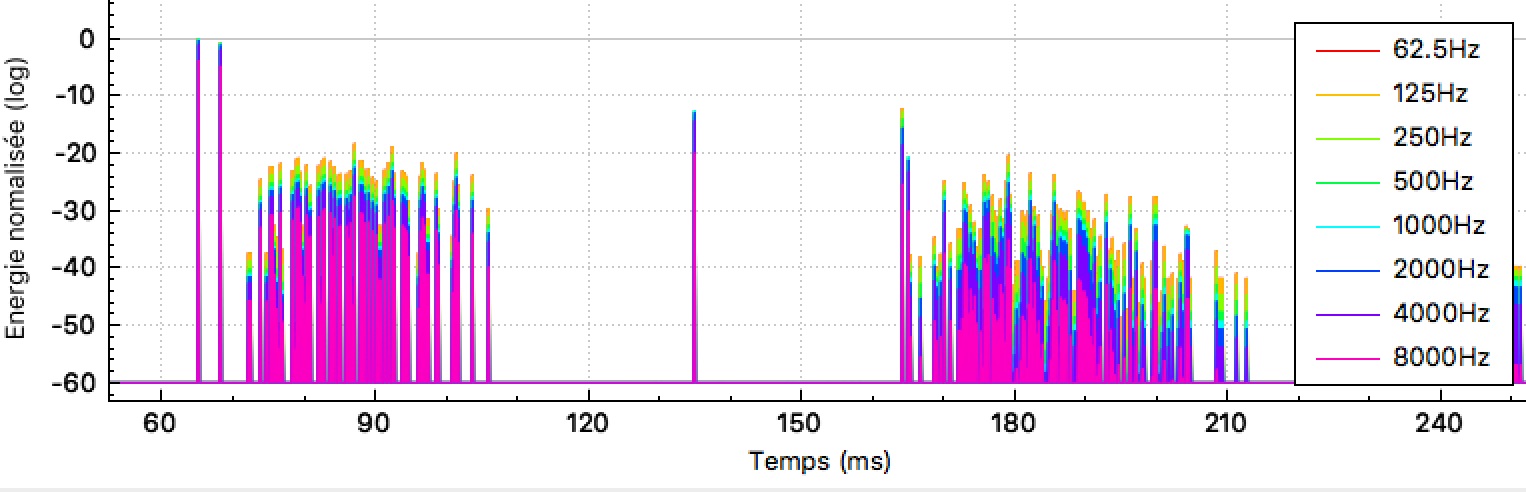
\includegraphics[width=\linewidth]{images/rirTheatrezoom}
		\caption{Zoom sur les premières réflexions}
		\label{rirTheatre30}
	\end{subfigureth}
	\caption{\gls{rir} du théâtre d'Orange dans sa configuration initiale pour 1million de rayons.}
	\label{rirTheatre}
\end{figureth}

La figure \ref{rirTheatre} illustre le fait que le \gls{RT60} est atteint en 2 secondes environ et le RT30 en 200ms. Cela montre que l'on passe rapidement en champs diffus mais que néanmoins il semble y avoir un léger écho perceptible à l'oreille (la sensibilité de l'oreille est de l'ordre de 50ms) au tout début du signal. Il y deux pics très rapprochés qui correspondent au son direct et à la réflexion sur l'orchestre. Il y a ensuite beaucoup de signal dispersé sur environ 50ms qui correspond aux rayons réfléchis sur le dossier des gradins et qui reviennent converger sur le récepteur. Le grand pic à -12dB est crée par la niche voutée centrale qui joue le rôle d'un miroir convergeant sur le récepteur. Les pics postérieurs sont le résultat de la forme semi-circulaire de la \gls{cavea} (voir fig. \ref{si_configInitale}). Le dernier pic de la figure \ref{rirTheatre30} semble être du aux réflexions sur le bas de la porte royale et la scène. 

\begin{figureth}
	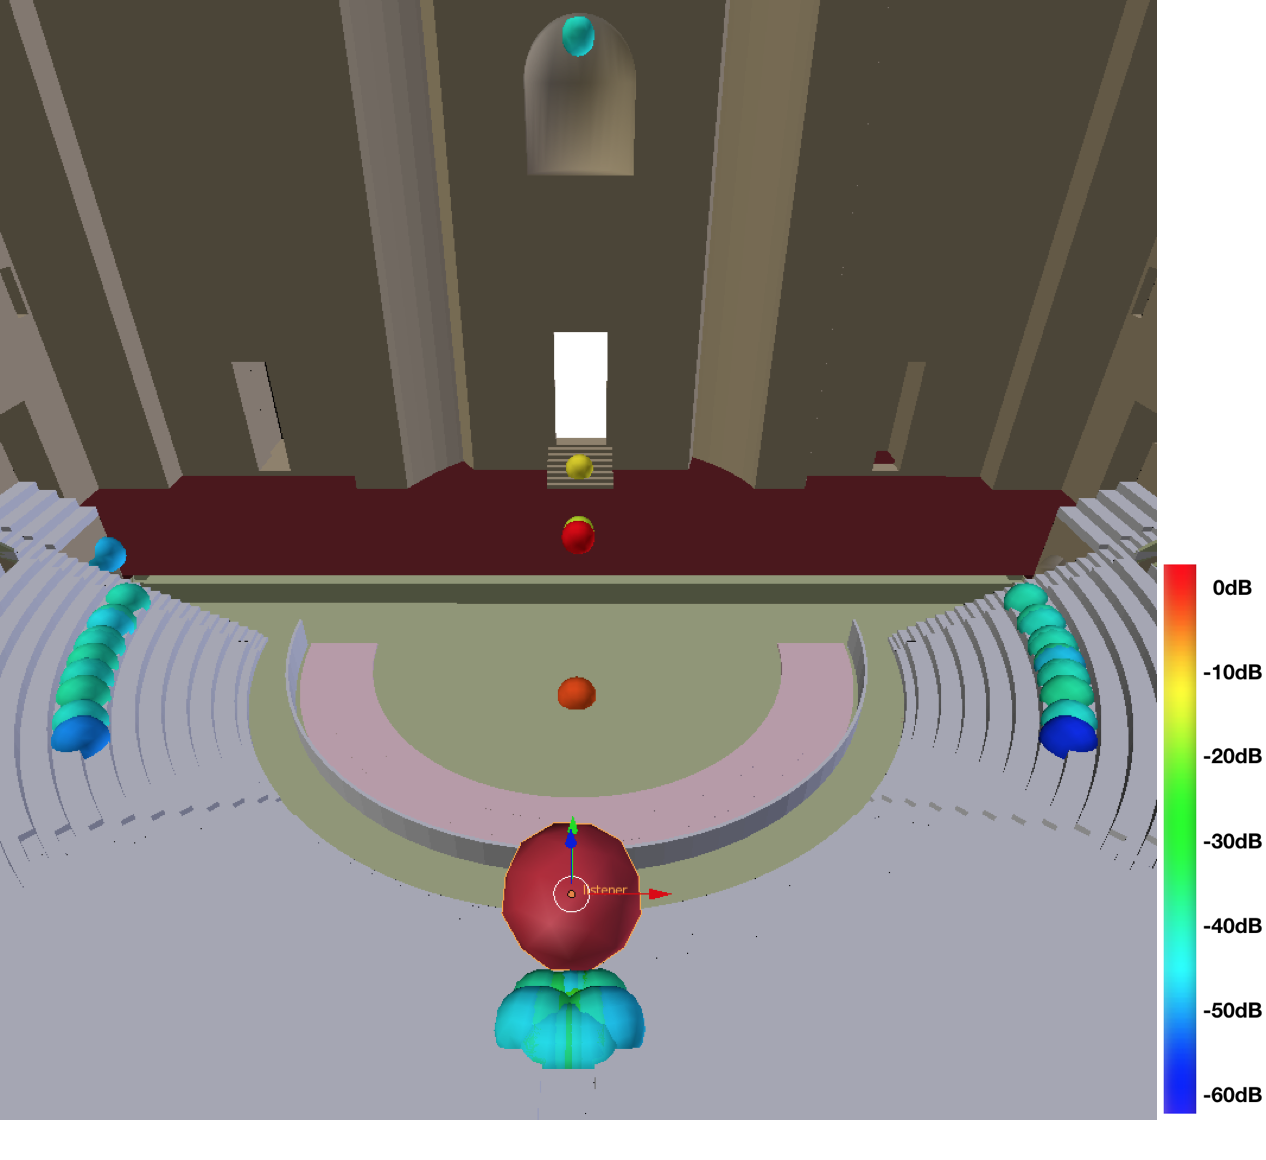
\includegraphics[width=0.8\linewidth]{images/si_configInitale}
	\caption{Première source-images projetée sur les parois du théâtre. Rouge correspond à l'énergie maximal et bleu l'énergie minimale}
	\label{si_configInitale}
\end{figureth}

A partir de cette analyse pour allons pouvoir procéder par comparaison avec cette configuration initiale pour déterminer l'impact des modifications apportées au bâtiment sur l'acoustique.
		
	\chapter{Test de configurations}
		\citationChap{
	Don't stop me now \\
	I'm having such a good time
			}{Queen}
		\minitoc
		\newpage
	
		\section{Position des spectateurs}
			\subsection{Devant}
			\subsection{Derrière}
			\subsection{Jardin}
			\subsection{Cours}
		\section{Forme du mur de scène}	
		\section{Présence de spectateurs}
		\section{Présence de velum}
		\section{Présence de la \gls{porticus isc}}
		\section{Forme et matériaux du toit}
		
		\newpage

	\chapter{Comparaison avec d'autres théâtres antiques}
		\citationChap{
		Si on veut connaitre un peuple, il faut écouter sa musique
		}{Platon}
		\minitoc
		\newpage
	
	\chapter*{Conclusion}
	\addcontentsline{toc}{chapter}{Conclusion}
	
		\newpage
		
% Biblio
 \bibliographystyle{francaissc}
 \bibliography{Part3/Biblio}
\addcontentsline{toc}{chapter}{Références}
